\documentclass{article}
\usepackage[utf8]{inputenc}
\usepackage{hyperref}
\usepackage{graphicx}
\usepackage{amsmath, amssymb}
\graphicspath{ {./images/} }

\title{SOLVING ONE DIMENSIONAL POISSON EQUATION
FYS 4150 – COMPUTATIONAL PHYSICS
}
\author{Jeyalakshmi Thoppe Subramanian }

\usepackage{natbib}


\begin{document}

\maketitle
\url{https://github.com/jeyalakt/4150COMP_PHY.git}
\section{Abstract}
In this Project one dimensional Poisson equation with Drichlet boundary conditions is solved with two algorithms -Gaussian Elimination and LU decomposition . It is observed that Gaussian elimination algorithm consumes less time and hence efficient than the LU decomposition. LU decomposition algorithm was used via pre built library function could not be used  for discretion values above in the order of 10000 while Gaussian elimination algorithm can be used .

\section{Introduction}
Poisson equation describes the electrostatic potential generated by localised charge distribution in electromagnetism  . This study intents  to solve  the Poisson equation using two different algorithms -first,  Gaussian elimination algorithm and second LU decomposition method.
We study how these two algorithms are used to solve the Poisson equation at different precision levels and how Gaussian elimination is more efficient that LU decomposition method.
First, the how the second derivative of  Poisson equation  can be approximated to 3 point formula is presented followed by elaboration on the proposed algorithms .Then the results of the algorithms are presented . Finally, a brief discussion on the results and remarks are provided.
\section{Theory}
The Poisson equation 
In electromagnetism, the poisson equation describes the electrostatic potential $\Phi$ generated by localised charge distribution $\rho(r)$
by 
\begin{equation}
\delta^2 \phi = -4\pi\rho(r)\label{1}
\end{equation}
in three dimensions.

In this study , we assume spherical symmetry of $\Phi$ and $\rho(r)$, as
\begin{equation}
\frac{1}{r^2}\frac{d}{dr}(\frac{r^2 d\phi}{dr})
\end{equation}

substituting  $\Phi$(r) with $\frac{\Phi(r)}{r}$
\begin{equation}
\frac{d^2\phi}{dr^2}= -4\pi\rho(r)
\end{equation}
Letting $\phi\rightarrow u$  and $r\rightarrow x$ , this equation simplifies as
\begin{equation}
-u''(x) = f(x).
\end{equation}


The homogeneous term f or source term is given by the charge distribution $\rho(r)$ and constant $-4\phi$
However in this study the source term form is taken as 
\begin{equation}
func{x}=100\exp{-10x}
\end{equation}

and results will be compared with numerical solution of 
\begin{equation}
u(x) = 1-(1-e^{-10})x-e^{-10x}
\end{equation}

in this project we try t solve the one dimensional Poisson equation with Dirichlet boundary condition 

\begin{equation}
-u''(x) = f(x), \hspace{0.5cm} x\in(0,1), \hspace{0.5cm} u(0) = u(1) = 0.
\end{equation}


\section{Approximation of second derivative}

in this study , the one dimensional Poisson equation is solved with Dirichlet bundary condition by rewriting it as set of linear equations.

The discretised approximation of u is defiend as vi with discretion or grid points 
xi=ih , step sixe h =1/n in the interval x0= 0 to xn=1 with boundary conditions v0=0 and vn = 0
n is normally taken in multiples of 10 
As the boundary conditions are fixed they are ignored and only the interior solution vi£(1...n) needs to be found.

The second derivative of equation 4 is approximated as 3 point formula
bt
\begin{equation}
   -\frac{v_{i+1}+v_{i-1}-2v_i}{h^2} = f_i  \hspace{0.5cm} \mathrm{for} \hspace{0.1cm} i=1,\dots, n,
\end{equation}
!et
where $f_i=f(x_i)$.

with $f$ is defined as $f = h^2 fi$
the equation can be rewritten as 
\begin{equation}
   -\frac{v_{i+1}+v_{i-1}-2v_i}{h^2} = f_i  \hspace{0.5cm} \mathrm{for} \hspace{0.1cm} i=1,\dots, n,
\end{equation}
!et
where $f_i=f(x_i)$

which can be represented in matrix equation 
\begin{equation}
   \mathbf{A}\mathbf{v} = \tilde{\mathbf{b}},
\end{equation}




\section{ algorithms}
Two algorithms are used to solve eqn 10 and the results are compared.
Gaussian elimination of Tridiagonal matrix A is used first . This method for Tridigonal matrix is called as Thomas algorithm. [1]
The second methos is LU decomposition
Complete programs in C++ and plotting of results in python program is given in the git hub link 
\section{ Gaussian elimination algorithm}
Notes from the github repository of computational physics for linear algorithms [2] are used to solve.
Matrix A in 11 is written in general form as
\[
    \mathbf{A} = \begin{bmatrix}
                           2& -1& 0 &\dots   & \dots &0 \\
                           -1 & 2 & -1 &0 &\dots &\dots \\
                           0&-1 &2 & -1 & 0 & \dots \\
                           & \dots   & \dots &\dots   &\dots & \dots \\
                           0&\dots   &  &-1 &2& -1 \\
                           0&\dots    &  & 0  &-1 & 2 \\
                      \end{bmatrix},
\]

this is solved in two steps 
Forward substitution as follows :












the final solution is given by step two ,
backward substitution 






where i is from 1 to n-2

teh time taken for  this algorithm is calculated for different step size of n as the algorithm is run for various vlues of n 


\section{Snippets of algorithms}


\section{Results}
The results in terms of step size , exact function , numerical solution , relative error are stored in a file for each value of n .
CPU time comparision 
The timings of the algorithms were observed to be of the following order
( Note: timing  includes memory read and write and on the other tasks being processed by CPU at that time  )

\begin{figure}[h!]
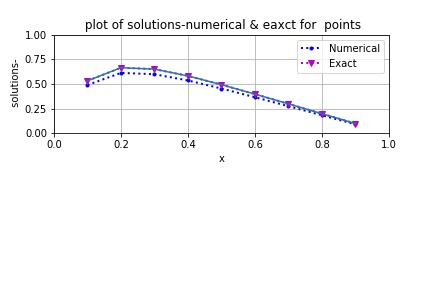
\includegraphics{gaussop1}
\centering
\caption{ Plot of exact and numerical solution by Gaussian Elimination algorithm for n=10 points}
\label{}
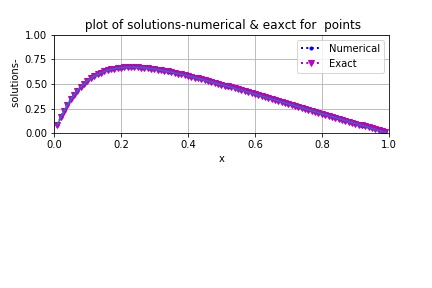
\includegraphics{gaussop2}
\centering
\caption{ Plot of exact and numerical solution by Gaussian Elimination algorithm for n=100 points}
\label{}
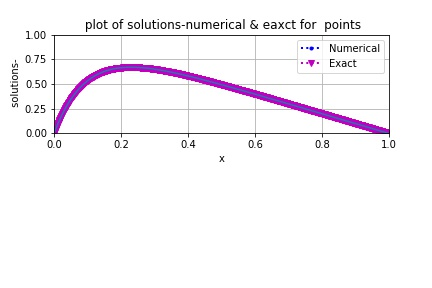
\includegraphics{gaussop3}
\centering
\caption{Figure 3 : Plot of exact and numerical solution by Gaussian Elimination algorithm for n=1000 points}
\label{}
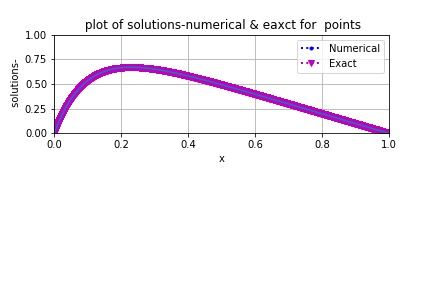
\includegraphics{gaussop4}
\centering
\caption{Figure 4 : Plot of exact and numerical solution by Gaussian Elimination algorithm for n=10000 points}
\label{}
\end{figure}
\section{Discussion}

Normally we intend to choose large value for n , assuming that it will result in higher precision .But from figure 5 (for gaussian elimination algorithm )we observe that this is true upto certain value of n only . This is due to loss of precision in numerical representation in the computer.A suitable value of n =105 gives results at reasonable cost of CPU time and memory 
Also the LU decomposition algorithm consumes 8*1010  bytes (app. 80 GB) of memory for value n=105   which strongly affects our ability performing the calculation.
So Gaussian elimination method is found more efficient.
\section{Conclusion}
The results show the importance of choosing suitable algorithm before solving a problem numerically within the constraints of time and memory and at reasonably accepted precision. Loss of numerical precision in numerical representation in computer also needs to to be considered.
In this study it is found that Gaussian elimination algorithm is more efficient than LU decomposition .
\section{References} 
\bibliographystyle{plain}
\bibliography{references}
@{ {Thomas, L.H. },
{ Elliptic Problems in Linear Differential Equations over a Network.
Watson Sci. Comput. Lab Report, Columbia University, New York. },
{1949}
}

@{ {Hjorth-Jensen, M.  },
{Computational Physics - Lecture Notes 2015. University of Oslo },
{2015}
}

@{ {Hjorth-Jensen, M. },
{Computational Physics-documents- linear algorithms. University of Oslo},
{2015}
}
\end{document}
